\setcounter{chapter}{1}
\chapter{Introducción al Problema y Necesidad}
Este capítulo analiza el problema y las necesidades de la Marina y Club Náutico Bahía Panitao S.A., a partir de los antecedentes operacionales, las entrevistas y las exigencias contenidas en las Bases Técnicas del Caso 07. Presenta una síntesis del problema, explica sus causas y consecuencias, identifica a los actores afectados y sus intereses. También distingue los requerimientos del cliente, los supuestos, exclusiones y restricciones que afectan al proyecto.

El diagnóstico fundamenta el alcance que se desarrolla en el Subdocumento 3 y las decisiones de arquitectura y datos de los Subdocumentos 4 y 5. Los listados detallados de requerimientos, supuestos, exclusiones y restricciones se presentan en el archivo SYNAPTIX-Subdocumento2-Anexos. Este capítulo concentra su desarrollo en entender la situación del cliente y los resultados que debe alcanzar.

\newpage
%---------------------------------------
\section{Resumen Ejecutivo del problema} %2.1
La Marina y Club Náutico Bahía Panitao S.A., ubicada en Puerto Montt, reúne servicios de amarra, invernada, varadero, combustible, escuela de vela y actividades de club. Administra 320 amarras y recibe anualmente a 640 alumnos de vela, incluidos 470 menores de edad. El 68\,\% de su actividad se concentra entre el 15 de noviembre y el 31 de marzo, período que intensifica la coordinación entre áreas \parencite[cap.~2, seccs.~2.1-2.2, pp.~5-6]{pucv-caso07-2026}.

El problema central es la dificultad para conocer y demostrar el estado de la operación. Los contratos, servicios y movimientos se registran en cuadernos, planillas y sistemas aislados. Para reunir esos antecedentes, las áreas dependen de consultas manuales y del conocimiento de personas específicas. El sistema administrativo no recibe soporte desde 2021 y una sola persona sabe ejecutar su cierre mensual. Esta fragmentación dificulta coordinar actividades, respaldar cobros y reconstruir quién actuó, cuándo y con qué resultado \parencite[caps.~4-5, pp.~9-14]{pucv-caso07-2026}.

Las consecuencias afectan la seguridad, la custodia y el control económico y ambiental. En la marejada de julio de 2026 no existía evidencia suficiente de los avisos realizados. En la escuela, establecer que un alumno había sido retirado antes de la clase tomó 40 minutos, aunque el menor no estuvo en peligro. A ello se suman dos personas dedicadas cinco días al mes a reunir antecedentes para facturar, un 6\,\% de documentos corregidos mediante notas de crédito por error y tres no conformidades ambientales que deben cerrarse para la temporada 2029 \parencite[cap.~1, pp.~4-5; cap.~4, secc.~4.11, p.~13; cap.~18, criterio~19, p.~44]{pucv-caso07-2026}.

Los afectados son el personal de operaciones y administración, la escuela, los alumnos y sus apoderados, los armadores y los contratistas. La gerencia debe responder por sus necesidades en una organización sin personal propio de tecnologías de información. El cliente requiere información oportuna sobre personas, embarcaciones y servicios, junto con responsabilidades de registro y validación que pueda sostener. El éxito depende de integrar esos registros al trabajo real del puerto, respetando la seguridad de las maniobras y la privacidad de los participantes \parencite[cap.~2, secc.~2.4, pp.~7-8; cap.~10, p.~26]{pucv-caso07-2026}.

%---------------------------------------
\newpage
\section{Comprensión del problema y de la necesidad} %2.2
\label{sec:comprension_problema}

El problema de la Marina y Club Náutico Bahía Panitao S.A. surge de la relación entre sus procesos, las condiciones del trabajo y la forma en que se conserva y comparte la información. Las dificultades descritas en las bases afectan la coordinación cotidiana, el control de los servicios y la capacidad de demostrar las actuaciones realizadas. Este apartado examina el contexto operacional, las causas de esas dificultades y las necesidades que se desprenden de ellas. Su magnitud se desarrolla en el apartado~\ref{sec:dimensionamiento_problema}.

\subsection{Contexto organizacional y sectorial} %2.2.1
La siguiente caracterización se basa en los antecedentes de la compañía, sus instalaciones, procesos y condiciones de conectividad descritos en las Bases Técnicas del Caso 07 \parencite[caps.~1-6, pp.~4-15]{pucv-caso07-2026}.
A partir de ellos, se analizan las relaciones entre servicios, las condiciones de trabajo y sus consecuencias para la gestión de información.

La marina combina servicios que comparten instalaciones y personal, pero tienen responsabilidades y ciclos distintos. Una embarcación puede mantener un contrato de amarra, recibir combustible e ingresar al varadero. Cada actividad genera antecedentes que administración debe relacionar para respaldar los cobros. Por esto, la coordinación exige vincular contratos, situación de la embarcación y servicios efectivamente prestados \parencite[cap.~4, pp.~9-13]{pucv-caso07-2026}.

La capacidad disponible tampoco se determina contando puestos libres. Una amarra debe ser compatible con las dimensiones y el calado de la embarcación, mientras que la ubicación en invernada condiciona el orden de salida. Es necesario distinguir ocupación física, asignación operacional y compromiso contractual: una salida temporal no libera necesariamente el puesto para otro cliente \parencite[cap.~3, p.~8; cap.~4, seccs.~4.1 y 4.6, pp.~9 y 11]{pucv-caso07-2026}.

Las condiciones de terreno determinan cuándo y cómo puede registrarse información. Los pantalanes están expuestos a humedad, salinidad y movimiento; el varadero opera con cargas suspendidas; y el surtidor impone restricciones por el manejo de combustibles. El campo de boyas de Bahía Ilque carece de energía, conectividad y personal permanente. El registro debe respetar los momentos seguros de trabajo y los períodos sin comunicación, manteniendo la radio marítima como medio de coordinación operacional \parencite[cap.~3, p.~8; cap.~6, pp.~14-15]{pucv-caso07-2026}.

La temporada alta incorpora trabajadores que deben aprender procedimientos apoyados en la experiencia del personal permanente. Las marejadas, además, obligan a suspender actividades y reorganizar agendas y avisos. Estas condiciones aumentan la necesidad de procedimientos claros y antecedentes accesibles. Sus magnitudes se desarrollan en el apartado~\ref{sec:estacionalidad_crecimiento}. La ausencia de personal TI exige, a su vez, distinguir la validación funcional del negocio de las tareas especializadas de soporte y recuperación \parencite[cap.~2, seccs.~2.2 y 2.4, pp.~6-8; cap.~4, secc.~4.5, pp.~10-11]{pucv-caso07-2026}.

El entorno sectorial incorpora exigencias de operación marítima, combustibles, residuos, documentación, seguros y certificación ambiental. Estas materias requieren evidencia, pero mantienen atribuciones diferentes: preparar los antecedentes de zarpe no equivale a otorgarlo, y respaldar una auditoría ambiental no equivale a certificar la marina. En la escuela, la participación de menores exige relacionar autorizaciones, retiros, salidas y monitores responsables, con acceso restringido a los datos personales pertinentes \parencite[cap.~2, secc.~2.1, p.~5; cap.~4, seccs.~4.3-4.9, pp.~10-12; cap.~10, p.~26; cap.~12, pp.~27-28; cap.~15, RT-16.09, p.~35]{pucv-caso07-2026}.

La calidad de la información también condiciona la relación comercial con la operadora internacional de charter. Su renovación depende de servicios en línea, atención mediante una interfaz en inglés, facturación por consumos reales y mantenimiento de la certificación ambiental. Los registros deben, por tanto, respaldar tanto el control interno como los compromisos asumidos frente a los clientes \parencite[cap.~1, pp.~4-5]{pucv-caso07-2026}.

\subsection{Situación actual, causas y consecuencias} %2.2.2

El diagnóstico identifica cuatro debilidades relacionadas: registros dispersos, cambios de estado no compartidos, antecedentes desactualizados y conocimiento concentrado en personas específicas. La Figura~\ref{fig:causas_consecuencias} presenta relaciones representativas entre estas causas, las brechas que producen y sus consecuencias. Se trata de una síntesis analítica de Synaptix basada en los antecedentes del caso.

\begin{figure}[htbp]
    \centering
    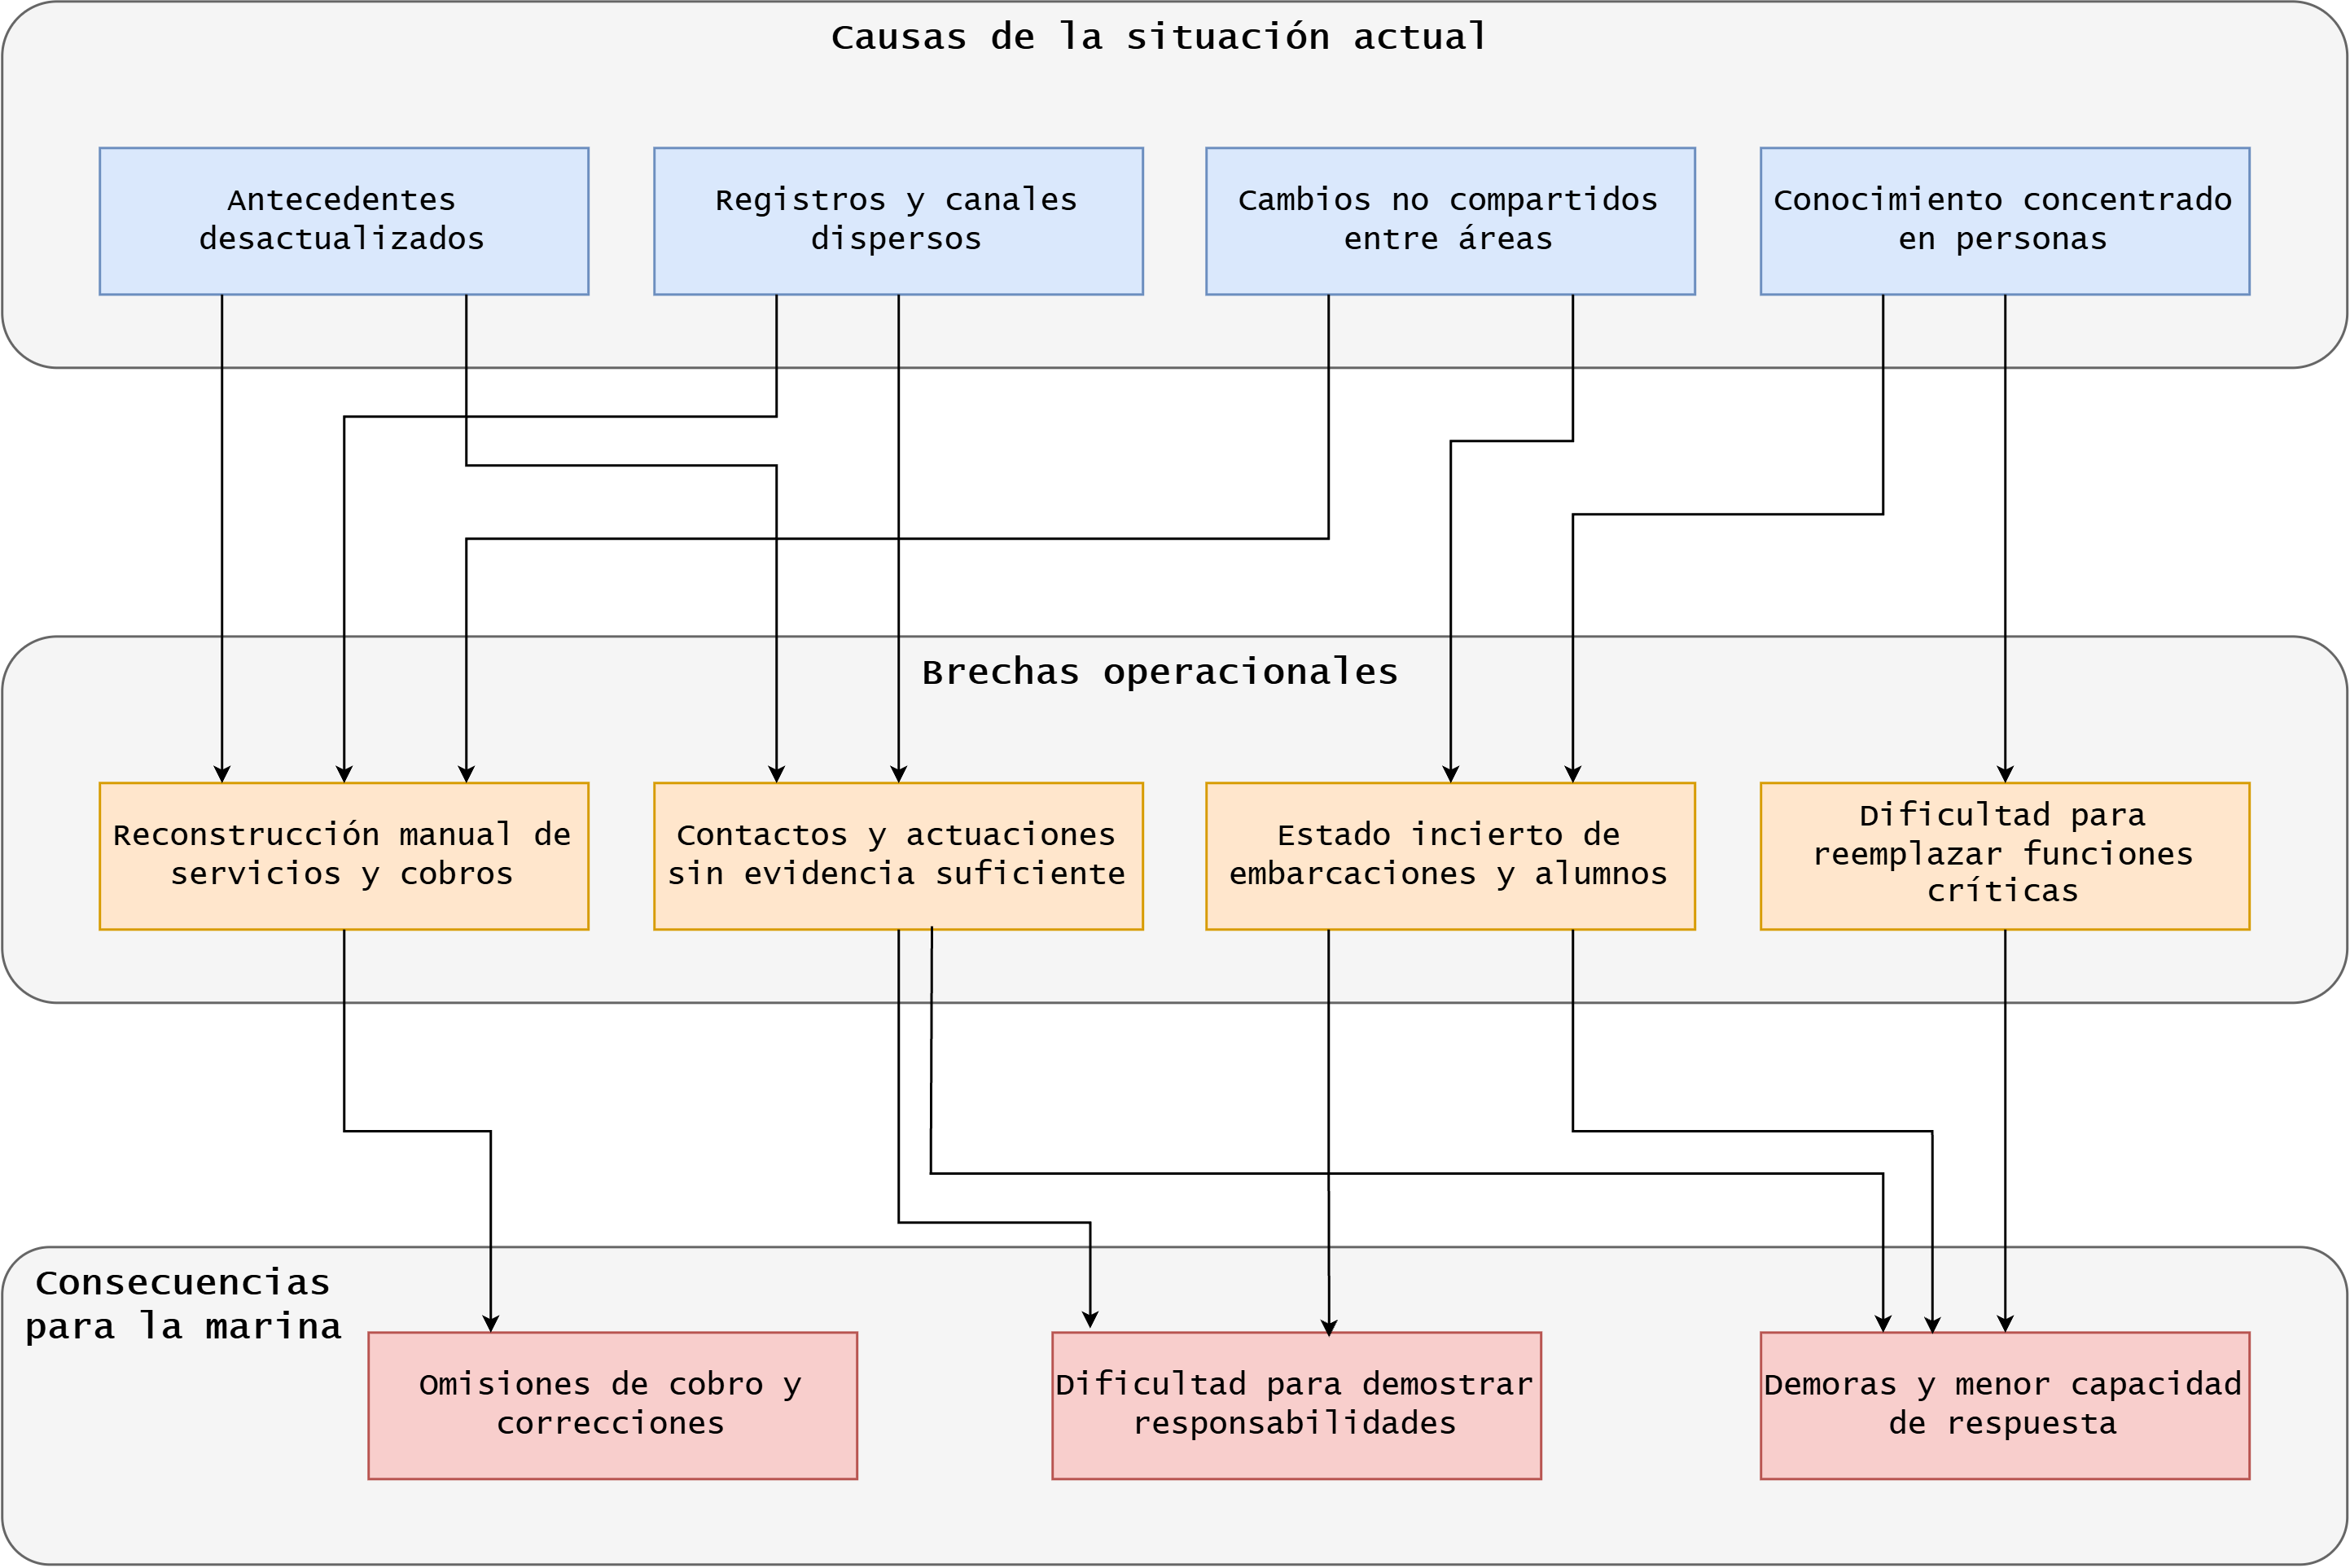
\includegraphics[width=\linewidth]{figuras/CausaConsecuencia.png}
    \caption{Relación entre causas, brechas operacionales y consecuencias}
    \label{fig:causas_consecuencias}
    \par\fontsize{9}{12}\selectfontskip
    \begin{minipage}{\linewidth}
        \fontsize{9}{12}\selectfont \FuenteFigura{\parencite[caps.~4-7, pp.~9-17]{pucv-caso07-2026}.}
    \end{minipage}
\end{figure}

Las relaciones no son exclusivas: varias causas pueden contribuir a una misma consecuencia. Por ejemplo, un cobro incorrecto puede originarse en un servicio omitido o en antecedentes contractuales desactualizados. Las principales manifestaciones se describen a continuación.

\textbf{Fragmentación entre áreas:}
Las reservas llegan por distintos canales, la asignación de amarras depende de un plano manual y los servicios se informan mediante cuadernos y anotaciones. Cada área conserva una parte del proceso, cuya reconstrucción exige consultas adicionales. Esto dificulta comprobar la disponibilidad de un puesto y vincular cada prestación con la embarcación y las condiciones de cobro correspondientes \parencite[cap.~4, seccs.~4.1-4.3 y 4.11, pp.~9-10 y 12-13]{pucv-caso07-2026}.

\textbf{Cambios de estado no compartidos:}
La marina tramita salidas, pero no registra sistemáticamente los regresos; los planes voluntarios se archivan sin seguimiento posterior. En la escuela, los retiros registrados en portería no actualizan oportunamente la información de los monitores. En las boyas, las observaciones se comunican al volver de la inspección. La información puede existir localmente y no estar disponible para quien pueda necesitarla. La falta de confirmación de regreso no demuestra que una embarcación siga navegando, del mismo modo que la asistencia inicial no acredita la participación efectiva de un alumno en una salida \parencite[cap.~4, seccs.~4.4, 4.9 y 4.10, pp.~10-12]{pucv-caso07-2026}.

\textbf{Antecedentes desactualizados y evidencia incompleta:}
Los contactos obsoletos limitan los avisos de marejada y las correcciones documentales agregan trabajo al zarpe. Además, realizar una actuación no asegura que quede constancia de su responsable, momento, resultado o autorización. La misma brecha afecta la trazabilidad ambiental cuando no se relacionan el origen y el destino de los residuos. Esto dificulta tanto la respuesta inmediata como la reconstrucción posterior ante reclamos, aseguradoras o auditorías \parencite[cap.~4, seccs.~4.3, 4.5 y 4.7, pp.~10-11]{pucv-caso07-2026}.

\textbf{Dependencia de personas específicas:}
Dos personas concentran el conocimiento de los puntos de izaje y una sola sabe ejecutar el cierre mensual del sistema administrativo. A ello se suman la falta de soporte desde 2021 y la ausencia de una fecha registrada para la última restauración verificada de respaldos \parencite[cap.~4, secc.~4.6, p.~11; caps.~5-6, pp.~13-15]{pucv-caso07-2026}.



\subsection{Necesidades del cliente y condiciones de éxito} %2.2.3

Las necesidades del cliente se agrupan en tres resultados operacionales: conocer el estado de personas y embarcaciones, relacionar los hechos con sus efectos administrativos y ambientales, y sostener procedimientos compatibles con la organización. Estas condiciones permiten evaluar la mejora sin anticipar su arquitectura.

\textbf{Conocer el estado operacional y resolver discrepancias:}
La marina necesita distinguir puestos ocupados, asignados y disponibles; salidas y regresos registrados; y participación efectiva de los alumnos. El éxito requiere reconocer el origen y la oportunidad de cada antecedente, identificar situaciones pendientes de confirmación y asignar responsables para revisarlas. También exige disponer de los antecedentes de izaje antes de la maniobra. Además, en caso de emergencias, se deben diferenciar los avisos enviados, los contactos confirmados y las autorizaciones recibidas \parencite[cap.~4, seccs.~4.1, 4.4-4.6 y 4.9, pp.~9-12; cap.~18, criterio~14, p.~44]{pucv-caso07-2026}.

\textbf{Relacionar servicios, registros y efectos administrativos:}
Cada servicio debe vincularse con la embarcación, el contrato y los antecedentes de cobro correspondientes. Del mismo modo, los residuos deben relacionarse con su origen y entrega al gestor, los consumos con el servicio y los avisos con sus destinatarios y resultados. El éxito consiste en reconstruir esas relaciones y aclarar diferencias con evidencia. La mejora del registro apoya la cobranza y la gestión ambiental, pero recuperar deudas o cerrar no conformidades también depende de decisiones y actuaciones del cliente \parencite[cap.~4, seccs.~4.5, 4.7 y 4.11-4.12, pp.~10-13]{pucv-caso07-2026}.

\textbf{Sostener procedimientos viables para la organización:}
El personal permanente, estacional y externo necesita saber qué registrar, cuándo hacerlo y a quién informar una discrepancia. Los procedimientos deben respetar los momentos seguros de trabajo y conservar los hechos durante las interrupciones de comunicación. Su continuidad requiere responsables funcionales para validar los antecedentes y un servicio especializado para las tareas técnicas que la marina no puede asumir. Una condición de éxito es reducir la dependencia de cuadernos paralelos y de personas específicas, sin interferir con amarres, izajes o actividades de la escuela \parencite[cap.~2, secc.~2.4, pp.~7-8; cap.~10, p.~26; cap.~15, RT-03.10, p.~33]{pucv-caso07-2026}.

El apartado~\ref{sec:dimensionamiento_problema} establece la magnitud de estas necesidades, el apartado~\ref{sec:actores_interes} identifica a los participantes y sus tensiones, y el apartado~\ref{sec:requerimientos_supuestos} sintetiza las exigencias y los límites que debe respetar la propuesta.

%---------------------------------------
\newpage
\section{Dimensionamiento del problema} %2.3
\label{sec:dimensionamiento_problema}
Este apartado dimensiona el problema del negocio en tres aspectos: la escala de la operación, las brechas detectadas y los períodos en que se concentran las actividades.

Las cifras utilizadas provienen de las Bases Técnicas del Caso 07. Por lo tanto, corresponden a antecedentes del diagnóstico y no a mediciones realizadas por Synaptix. Cuando se presentan resultados calculados a partir de estas cifras, se indica cómo se obtuvieron y de qué manera deben interpretarse. Para evitar confusiones, las capacidades físicas, los volúmenes de actividad, la cantidad de participantes y los episodios se analizan por separado. Además, los cálculos derivados no representan ahorros comprometidos, ni deben interpretarse directamente como usuarios simultáneos o transacciones del sistema.

La traducción de este dimensionamiento a requerimientos de capacidad tecnológica y volúmenes de datos se desarrolla en los Subdocumentos 4 y 5.

\subsection{Escala y capacidad operacional} %2.3.1

La magnitud del puerto combina capacidad física, actividad anual y participación de personas y empresas. Una amarra representa una unidad de capacidad física, mientras que una recalada o un movimiento de izaje corresponde a una actividad realizada durante un período. La Tabla~\ref{tab:escala_operacion} reúne las principales magnitudes que permiten contextualizar el diagnóstico.

\begingroup
\setlength{\tabcolsep}{3pt}

\begin{longtable}{@{}L{.15\textwidth}L{.30\textwidth}>{\raggedleft\arraybackslash}p{.19\textwidth}L{\dimexpr.36\textwidth-18pt\relax}@{}}
    \caption{Escala de la operación del puerto deportivo}
    \label{tab:escala_operacion}\\
    \hline
    \EncabezadoTabla{Dimensión} & \EncabezadoTabla{Indicador} & \EncabezadoTabla{Magnitud} & \EncabezadoTabla{Período o alcance} \\
    \hline
    \endfirsthead
    \hline
    \EncabezadoTabla{Dimensión} & \EncabezadoTabla{Indicador} & \EncabezadoTabla{Magnitud} & \EncabezadoTabla{Período o alcance} \\
    \hline
    \endhead
    Capacidad & Amarras en el agua & 320 & Recinto principal \\ \addlinespace \hline
    Capacidad & Puestos de invernada & 180 & 152 ocupados en invierno de 2026 \\ \addlinespace \hline
    Capacidad & Boyas de fondeo & 40 & Bahía Ilque \\ \addlinespace \hline
    Actividad & Zarpes tramitados & $\approx 4.800$ & Anuales \\ \addlinespace \hline
    Actividad & Recaladas de visitantes & $\approx 1.900$ & Anuales \\ \addlinespace \hline
    Actividad & Movimientos de travelift & 1.150 & Anuales \\ \addlinespace \hline
    Actividad & Combustible expendido & 1.900.000 litros & Anuales \\ \addlinespace \hline
    Participación & Alumnos de escuela de vela & 640 & Anuales; 470 menores de edad \\ \addlinespace \hline
    Participación & Empresas contratistas & 62 & Aproximadamente 140 personas \\ \addlinespace \hline
\end{longtable} \FuenteTabla{\parencite[cap.~2, seccs.~2.2-2.3, pp.~6-7; cap.~14, secc.~14.1, p.~31]{pucv-caso07-2026}.}
\endgroup

Las magnitudes muestran una operación diversa, cuyas unidades no son directamente equivalentes. El combustible expendido no determina la cantidad de despachos; una misma embarcación puede recalar varias veces, y una persona puede participar en más de un rol. Estas distinciones son necesarias para evitar que los volúmenes del negocio se conviertan, sin fundamento, en cantidades de usuarios o transacciones informáticas.

Como complemento, el caso registra 296 embarcaciones con contrato permanente de amarra y 1.240 socios del club. Los 28 puestos del muelle de espera y visitas están incluidos en las 320 amarras. La cantidad de contratos tampoco representa la ocupación física de un momento determinado, pues las embarcaciones pueden encontrarse navegando o en invernada \parencite[cap.~2, seccs.~2.2-2.3, p.~6]{pucv-caso07-2026}.

En la invernada, la utilización física durante el invierno de 2026 se obtiene al relacionar los 152 puestos ocupados con la capacidad total:

\begin{center}
$152 \div 180 \times 100 \approx 84{,}4$\,\% de ocupación.
\end{center}

Este resultado describe la utilización en ese período, pero no garantiza que los puestos restantes puedan ocuparse sin restricciones. La ubicación de cada embarcación condiciona las maniobras y el orden de salida. De forma similar, una amarra libre sólo puede asignarse después de considerar su compatibilidad y sus compromisos operacionales \parencite[cap.~3, p.~8; cap.~4, seccs.~4.1 y 4.6, pp.~9 y 11]{pucv-caso07-2026}.

La ocupación media anual de amarras es de 84\,\%, mientras en temporada alta alcanza 98\,\%. Estos valores describen las amarras y no deben confundirse con el 84,4\,\% de utilización de invernada calculado anteriormente. La diferencia temporal explica que exista capacidad media disponible y, a la vez, presión estacional; la compatibilidad y los compromisos de cada puesto condicionan cuánto de esa capacidad puede utilizarse \parencite[cap.~7, secc.~7.1, p.~15]{pucv-caso07-2026}.

El aprovechamiento de las amarras presenta un desajuste adicional: el 22\,\% de las contratadas está ocupado por embarcaciones cuya eslora no corresponde al tramo pagado, mientras 90 embarcaciones de esloras superiores a 15 metros permanecen en lista de espera. La diferencia tarifaria no demuestra por sí sola una incompatibilidad física, pero sí evidencia una relación insuficientemente controlada entre contratación, asignación y demanda. Por ello, aumentar la capacidad no resolvería necesariamente las dificultades de utilización que ya existen \parencite[cap.~4, secc.~4.1, p.~9]{pucv-caso07-2026}.

\subsection{Línea base e impactos del problema} %2.3.2

La escala debe relacionarse con las brechas que afectan la oportunidad, completitud y exactitud de la información. La Tabla~\ref{tab:indicadores_situacion_actual} presenta indicadores de la situación actual. Cada valor conserva el alcance del proceso o episodio descrito en las bases, sus porcentajes no deben sumarse porque son poblaciones diferentes.

\begingroup
\setlength{\tabcolsep}{3pt}

\begin{longtable}{@{}L{.15\textwidth}L{.43\textwidth}>{\raggedleft\arraybackslash}p{.17\textwidth}L{\dimexpr.25\textwidth-18pt\relax}@{}}
    \caption{Indicadores de la situación actual}
    \label{tab:indicadores_situacion_actual}\\
    \hline
    \EncabezadoTabla{Ámbito} & \EncabezadoTabla{Indicador} & \EncabezadoTabla{Línea base} & \EncabezadoTabla{Fuente del caso} \\
    \hline
    \endfirsthead
    \hline
    \EncabezadoTabla{Ámbito} & \EncabezadoTabla{Indicador} & \EncabezadoTabla{Línea base} & \EncabezadoTabla{Fuente del caso} \\
    \hline
    \endhead
    Amarras & Tiempo medio de asignación a visitantes & 11 minutos & Secc. 4.2, p.~9 \\ \addlinespace \hline
    Servicios & Recaladas sin registro facturable & 9\,\% & Secc. 4.2, p.~10 \\ \addlinespace \hline
    Zarpe & Tiempo por trámite & 18 minutos & Secc. 4.3, p.~10 \\ \addlinespace \hline
    Zarpe & Trámites con corrección manual & 34\,\% & Secc. 4.3, p.~10 \\ \addlinespace \hline
    Marejadas & Armadores contactados el 8 de julio de 2026 & 190 de 296 & Secc. 4.5, p.~11 \\ \addlinespace \hline
    Contactos & Contratos con algún contacto obsoleto & 47\,\% & Secc. 4.5, p.~11 \\ \addlinespace \hline
    Contratistas & Empresas con acreditación completa y vigente & 41\,\% & Secc. 4.7, p.~11 \\ \addlinespace \hline
    Facturación & Documentos con nota de crédito por error & 6\,\% & Secc. 4.11, p.~13 \\
\end{longtable} \FuenteTabla{\parencite[cap.~4, pp.~9-13]{pucv-caso07-2026}. La columna «Fuente del caso» identifica la sección y página correspondientes a cada indicador.}
\endgroup

Los indicadores muestran dificultades en etapas distintas: consultar disponibilidad, preparar documentos, contactar responsables, verificar acreditaciones y consolidar cobros. Su interpretación requiere considerar tanto el volumen afectado como las consecuencias de cada brecha. Por ejemplo, los once minutos de asignación implican espera mientras una embarcación permanece frente al acceso; una cobertura incompleta de avisos, en cambio, compromete la capacidad de coordinar medidas ante una contingencia.

Para precisar la magnitud de las actividades recurrentes y del episodio de marejada, la Tabla~\ref{tab:calculos_dimensionamiento} reúne los resultados derivados. En la tramitación del zarpe se utilizan 18 minutos por trámite y aproximadamente 4.800 trámites anuales; para la consolidación de facturación, las bases informan dos personas dedicadas durante cinco días al mes. Las estimaciones anuales aplican las tasas del caso a sus volúmenes aproximados, sin constituir nuevos recuentos observados.

\begingroup
\setlength{\tabcolsep}{3pt}

\begin{longtable}{@{}L{.50\textwidth}L{.27\textwidth}>{\raggedleft\arraybackslash}p{\dimexpr.23\textwidth-12pt\relax}@{}}
    \caption{Resultados derivados para dimensionar las brechas}
    \label{tab:calculos_dimensionamiento}\\
    \hline
    \EncabezadoTabla{Magnitud derivada} & \EncabezadoTabla{Cálculo} & \EncabezadoTabla{Resultado} \\
    \hline
    \endfirsthead
    \hline
    \EncabezadoTabla{Magnitud derivada} & \EncabezadoTabla{Cálculo} & \EncabezadoTabla{Resultado} \\
    \hline
    \endhead
    Tiempo anual de tramitación de zarpes & $4.800 \times 18 \div 60$ & $\approx 1.440$ horas/año \\ \addlinespace \hline
    Zarpes con corrección manual & $4.800 \times 0{,}34$ & $\approx 1.632$ trámites/año \\ \addlinespace \hline
    Cobertura de contacto en la marejada & $190 \div 296 \times 100$ & $\approx 64{,}2$\,\% \\ \addlinespace \hline
    Armadores no contactados en ese episodio & $296 - 190$ & 106 armadores \\ \addlinespace \hline
    Recaladas sin registro facturable & $1.900 \times 0{,}09$ & $\approx 171$ recaladas/año \\ \addlinespace \hline
    Esfuerzo mensual de consolidación para facturar & 2 personas $\times$ 5 días & 10 días-persona/mes \\ \addlinespace \hline
\end{longtable} \FuenteTabla{\parencite[cap.~2, secc.~2.2, p.~6; cap.~4, seccs.~4.2-4.3, pp.~9-10; secc.~4.5, pp.~10-11; secc.~4.11, pp.~12-13]{pucv-caso07-2026}.}
\endgroup

Los resultados permiten reconocer carga de trabajo, omisiones y cobertura, pero no representan beneficios ya obtenidos ni reducciones comprometidas. Las horas de tramitación incluyen actividades que seguirán siendo necesarias, y los días-persona expresan esfuerzo acumulado, no duración del cierre. Las implicaciones de cada ámbito se analizan a continuación.

\textbf{Preparación de zarpe y revisión documental:}
Las aproximadamente 1.440 horas anuales muestran la carga acumulada de un proceso que reutiliza de manera insuficiente antecedentes ya disponibles. Los cerca de 1.632 trámites con correcciones reflejan, además, la necesidad de revisar vigencias y cambios. No corresponde sumarles un tiempo adicional, porque las bases no indican la duración de esas correcciones ni si está incluida en los 18 minutos. La mejora debe centrarse en reducir trabajo repetido y errores, manteniendo las comprobaciones necesarias y las atribuciones de la autoridad marítima.

\textbf{Cobertura de avisos y capacidad de demostración:} El 64,2\,\% de contacto en la marejada deja 106 armadores sin contacto efectivo en ese episodio. Esta brecha se combina con la ausencia de evidencia sobre horarios, resultados e instrucciones. Contactar a una persona no demuestra por sí solo que haya autorizado una intervención o ejecutado medidas preventivas; esas actuaciones requieren registros propios. Asimismo, el 47\,\% de contratos con algún dato obsoleto no equivale al mismo porcentaje de armadores totalmente inubicables, porque pueden existir otros medios vigentes.

\textbf{Servicios facturables, cierre y cobranza:} Las aproximadamente 171 recaladas sin registro facturable representan actividad cuya consolidación administrativa es insuficiente. No permiten calcular una pérdida monetaria sin conocer permanencias, servicios y condiciones comerciales. Los diez días-persona mensuales de preparación muestran el esfuerzo de reunir antecedentes, mientras el 6\,\% de documentos con nota de crédito por error evidencia que esa reconstrucción no asegura la exactitud del resultado. El problema abarca tanto la completitud de los hechos registrados como su correcta interpretación para cobrar.

La cobranza agrega una dificultad que no se resuelve únicamente corrigiendo registros: el 11\,\% de los contratos está en mora y existen 14 embarcaciones abandonadas, con 26 meses de deuda promedio. Estas últimas ocupan capacidad y requieren antecedentes para respaldar las actuaciones del cliente. Disponer de información completa facilita su gestión, pero no equivale a recuperar automáticamente la deuda ni a poder disponer libremente de las embarcaciones \parencite[cap.~4, secc.~4.11, p.~13]{pucv-caso07-2026}.

\textbf{Escuela de vela y control de participación:} El volumen de 640 alumnos anuales, incluidos 470 menores de edad, da relevancia a la relación entre autorizaciones, asistencia, salidas y retiros. El episodio del 12 de enero de 2026 requirió 40 minutos para establecer que el alumno señalado como faltante había sido retirado antes de la clase. Ese tiempo corresponde a un incidente concreto y no constituye un promedio; tampoco representa un período de peligro efectivo, pues las bases señalan que el alumno no estuvo en riesgo. Su importancia es que los registros no permitieron responder oportunamente una pregunta esencial para la responsabilidad de la escuela \parencite[cap.~1, p.~4; cap.~2, secc.~2.2, p.~6; cap.~4, secc.~4.9, p.~12]{pucv-caso07-2026}.

\textbf{Varadero y preparación de maniobras:} Cada movimiento de travelift toma 74 minutos en promedio y ocupa a tres personas. Ese tiempo debe interpretarse junto con la seguridad y las condiciones de ejecución, por lo que no constituye un ahorro potencial directo. La brecha más relevante es la dependencia de dos personas para conocer los puntos de izaje. Los cuatro siniestros con daños registrados en cinco años refuerzan la importancia de disponer de antecedentes previos y evidencia de las actuaciones, sin demostrar que todos hayan sido causados exclusivamente por falta de información. El caso registra cero planes de izaje documentados para las 296 embarcaciones consideradas en ese indicador, lo que refuerza la dependencia del conocimiento personal \parencite[cap.~4, secc.~4.6, p.~11; cap.~7, secc.~7.3, p.~16]{pucv-caso07-2026}.

\textbf{Control ambiental y participación de terceros:} La acreditación completa y vigente alcanza al 41\,\% de las empresas contratistas; este porcentaje no debe aplicarse automáticamente a sus trabajadores. A su vez, el 38\,\% de costos de agua y energía no recuperados expresa una brecha económica, no una proporción de consumo desperdiciado. Las tres no conformidades ambientales se relacionan con trazabilidad de residuos, medición individual y evidencia de capacitación ambiental, con plazo de cierre para la temporada 2029. Su tratamiento requiere registros confiables y prácticas que permitan acreditar lo realizado. De siete derrames menores registrados en el año, dos cuentan con acta y seguimiento. Esta diferencia dimensiona una brecha de evidencia, sin demostrar que los demás no hayan recibido atención \parencite[cap.~1, pp.~4-5; cap.~4, seccs.~4.7 y 4.12, pp.~11-13; cap.~7, secc.~7.3, pp.~16-17; cap.~18, criterio~19, p.~44]{pucv-caso07-2026}.

Estas brechas tienen también una dimensión comercial: la operadora de charter mantiene 14 embarcaciones y representa el 22\,\% de los ingresos por amarra. Sus condiciones de renovación vinculan la atención y los consumos con la certificación ambiental. Este antecedente evidencia concentración de ingresos y exigencias de un cliente relevante; no representa una pérdida confirmada ni permite asignar una probabilidad de término de la relación \parencite[cap.~1, p.~5]{pucv-caso07-2026}.

Finalmente, algunos problemas se dimensionan por la ausencia de controles y por sus consecuencias, aunque no exista una tasa de error. Es el caso del registro sistemático de regresos, la asociación entre alumnos y embarcaciones y la evidencia de inspecciones de boyas. En estas últimas se informan dos desprendimientos en cuatro años sin registro de la última inspección del tren de fondeo correspondiente. La falta de porcentajes no reduce su importancia: muestra que la organización carece de antecedentes suficientes para evaluar de forma consistente su propio desempeño \parencite[cap.~4, seccs.~4.4, 4.9 y 4.10, pp.~10-12]{pucv-caso07-2026}.

\subsection{Estacionalidad y crecimiento} %2.3.3
\label{sec:estacionalidad_crecimiento}

La demanda no se distribuye uniformemente durante el año. Entre el 15 de noviembre y el 31 de marzo se concentra el 68\,\% de la actividad anual, mientras la dotación propia pasa de 39 a un máximo de 78 personas. La relación $78 \div 39 = 2$ muestra que el personal puede duplicarse cuando aumenta la carga de atención. Además, más de la mitad del refuerzo estacional de marineros es personal nuevo cada año, lo que incrementa la necesidad de procedimientos claros y antecedentes accesibles para quienes se incorporan \parencite[cap.~2, seccs.~2.2 y 2.4, pp.~6-7]{pucv-caso07-2026}.

El varadero presenta una concentración particular: el 62\,\% de los 1.150 movimientos anuales del travelift ocurre en dos campañas de seis semanas. La actividad conjunta se obtiene mediante \parencite[cap.~4, secc.~4.6, p.~11]{pucv-caso07-2026}:

\begin{center}
    $1.150 \times 0{,}62 = 713$ movimientos en ambas campañas.
\end{center}

Este resultado no implica una distribución idéntica entre campañas ni una carga diaria constante. Los atrasos, la marea, el viento y la posición de las embarcaciones pueden alterar la programación. El efecto de un retraso también alcanza a los trabajos posteriores, por lo que el volumen de movimientos debe interpretarse junto con sus dependencias y con la disponibilidad del equipo de izaje.

La simultaneidad entre servicios aumenta la presión sobre los puntos de atención. El capítulo 14 plantea una mañana de alta demanda, entre las 07:00 y las 11:00, con 90 zarpes, 20 recaladas de visitantes, tres clases en el agua y una campaña de varada. Este escenario permite examinar la coincidencia de actividades que necesitan coordinación y antecedentes vigentes. No debe tratarse como una jornada habitual ni utilizarse para modificar los volúmenes anuales; tampoco equivale directamente a una cantidad de transacciones informáticas \parencite[cap.~14, secc.~14.2, p.~33]{pucv-caso07-2026}.

Los eventos náuticos generan otra concentración puntual. El caso informa 14 regatas y eventos anuales, y señala que el mayor reúne 120 embarcaciones y hasta 800 personas en el recinto. Estas cifras describen asistencia y participación, no usuarios concurrentes de una aplicación. Su relevancia radica en el aumento de la coordinación de accesos, servicios y atención durante períodos específicos \parencite[cap.~2, secc.~2.2, p.~6]{pucv-caso07-2026}.

A estos ciclos se agregan las suspensiones por marejadas. Una interrupción puede obligar a modificar varias agendas y comunicar cambios a armadores, contratistas y participantes de la escuela. Por ello, el dimensionamiento debe considerar tanto la actividad programada como el trabajo de reorganización que se genera ante una contingencia. Dividir los totales anuales entre los días de operación ocultaría estas concentraciones \parencite[cap.~4, secc.~4.5, pp.~10-11]{pucv-caso07-2026}.

Finalmente, el cliente evalúa ampliar la capacidad a 380 amarras y 70 boyas entre 2031 y 2033. Respecto de la situación actual, los incrementos serían \parencite[cap.~15, RT-02.12, p.~33]{pucv-caso07-2026}:

\begin{center}
Amarras: $(380 - 320) \div 320 \times 100 = 18{,}75$\,\%.
\end{center}

\begin{center}
Boyas: $(70 - 40) \div 40 \times 100 = 75$\,\%.
\end{center}

Estos porcentajes corresponden a un escenario de expansión de capacidad física. No implican aumentos equivalentes de zarpes, servicios, registros o usuarios, cuyo crecimiento deberá justificarse por separado. En particular, la ampliación de boyas mantiene la necesidad de gestionar observaciones e inspecciones en un entorno separado del recinto principal.

El análisis muestra que la magnitud del problema depende del volumen de actividad, su concentración temporal y las consecuencias de la información incompleta. Una discrepancia durante una maniobra, una salida de alumnos o una contingencia puede exigir una respuesta inmediata, aunque involucre pocos registros. Estos antecedentes fundamentan las necesidades de coordinación, trazabilidad y continuidad que orientan los requerimientos del apartado~\ref{sec:requerimientos_supuestos}.

%---------------------------------------
\newpage
\section{Actores y Grupos de Interés} %2.4
\label{sec:actores_interes}

Los actores se identifican a partir de su participación en los procesos, de la información con la que interactúan y de su capacidad para influir en las decisiones del proyecto. Las entrevistas de las bases permiten reconocer necesidades coincidentes, pero también intereses que deben compatibilizarse para que la mejora resulte aceptable y sostenible \parencite[cap.~8, pp.~18-23]{pucv-caso07-2026}.


\subsection{Identificación de los actores} %2.4.1
La influencia representa la capacidad de un actor para aprobar decisiones, condicionar su aplicación, exigir cumplimiento o afectar la adopción de procedimientos. El interés expresa cuánto inciden los resultados del proyecto en sus actividades o responsabilidades. Las valoraciones alta, media y baja corresponden al análisis de Synaptix sobre las bases; no provienen de nuevas entrevistas.

La influencia se interpreta dentro del ámbito de cada participante: una jefatura puede condicionar la operación sin aprobar inversiones. Asimismo, un interés alto no supone apoyo automático al cambio; armadores y apoderados pueden valorar mejoras de seguridad y rechazar mecanismos que afecten su privacidad.

La Tabla~\ref{tab:actores_internos} distingue los ámbitos de responsabilidad y su influencia en el proyecto. El interés es alto en todos los grupos, porque el cambio afecta sus registros, procedimientos o decisiones; por ello, se declara aquí como condición común. En los grupos que reúnen jefatura y personal ejecutor, la influencia alta corresponde a la capacidad de la jefatura para definir y validar procedimientos, sin atribuir a todos sus integrantes la misma autoridad.

\begingroup
\setlength{\tabcolsep}{3pt}

\begin{longtable}{@{}L{.34\textwidth}L{.34\textwidth}L{.16\textwidth}L{\dimexpr.16\textwidth-18pt\relax}@{}}
    \caption{Valoración de actores internos}
    \label{tab:actores_internos}\\
    \hline
    \EncabezadoTabla{Actor o grupo} & \EncabezadoTabla{Ámbito principal} & \EncabezadoTabla{Influencia} & \EncabezadoTabla{Interés} \\
    \hline
    \endfirsthead
    \hline
    \EncabezadoTabla{Actor o grupo} & \EncabezadoTabla{Ámbito principal} & \EncabezadoTabla{Influencia} & \EncabezadoTabla{Interés} \\
    \hline
    \endhead
    Directorio y gerencia & Decisiones y sostenibilidad & Alta & Alto \\ \addlinespace \hline
    Jefatura de operaciones y torre & Coordinación marítima & Alta & Alto \\ \addlinespace \hline
    Marineros de pantalán & Observación y registro en terreno & Media & Alto \\ \addlinespace \hline
    Varadero y operadores de travelift & Programación y seguridad de izaje & Alta & Alto \\ \addlinespace \hline
    Escuela de vela y monitores & Participación y cuidado de alumnos & Alta & Alto \\ \addlinespace \hline
    Administración, atención a socios y cobranza & Contratos y control administrativo & Alta & Alto \\ \addlinespace \hline
    Portería y seguridad & Accesos, habilitación y retiros & Media & Alto \\ \addlinespace \hline
    Personal de combustible & Despachos y seguridad del surtidor & Media & Alto \\ \addlinespace \hline
    Mantenimiento e inspección de boyas & Estado e inspección de instalaciones & Media & Alto \\ \addlinespace
\end{longtable}

\FuenteTabla{\parencite[cap.~2, secc.~2.4, pp.~7-8; cap.~4, pp.~9-13; cap.~8, pp.~18-23]{pucv-caso07-2026}.}
\endgroup

Las diferencias de influencia responden a funciones distintas: directorio y gerencia condicionan prioridades y recursos; las jefaturas establecen criterios funcionales; y el personal de terreno determina la viabilidad práctica de los procedimientos. Estas responsabilidades no implican contar con soporte técnico especializado, pues la marina no dispone de personal TI.

La Tabla~\ref{tab:actores_externos} distingue a los clientes, participantes, terceros y entidades de fiscalización. Se separa la condición de cliente de la de accionista, así como la participación de los alumnos de la representación ejercida por sus apoderados.

\begingroup
\setlength{\tabcolsep}{3pt}

\begin{longtable}{@{}L{.34\textwidth}L{.34\textwidth}L{.16\textwidth}L{\dimexpr.16\textwidth-18pt\relax}@{}}
    \caption{Valoración de grupos de interés externos}
    \label{tab:actores_externos}\\
    \hline
    \EncabezadoTabla{Actor o grupo} & \EncabezadoTabla{Ámbito principal} & \EncabezadoTabla{Influencia} & \EncabezadoTabla{Interés} \\
    \hline
    \endfirsthead
    \hline
    \EncabezadoTabla{Actor o grupo} & \EncabezadoTabla{Ámbito principal} & \EncabezadoTabla{Influencia} & \EncabezadoTabla{Interés} \\
    \hline
    \endhead
    Armadores, socios y visitantes & Contratación y uso de servicios & Media & Alto \\ \addlinespace \hline
    Socios accionistas & Gobierno societario & Alta & Alto \\ \addlinespace \hline
    Operadora de charter & Continuidad comercial y servicios & Alta & Alto \\ \addlinespace \hline
    Apoderados y centro de padres & Autorizaciones y privacidad & Alta & Alto \\ \addlinespace \hline
    Alumnos de la escuela & Seguridad y participación & Baja & Alto \\ \addlinespace \hline
    Contratistas y sus trabajadores & Acreditación y trabajos en recinto & Media & Alto \\ \addlinespace \hline
    Gestor autorizado de residuos & Evidencia de recepción y destino & Media & Medio \\ \addlinespace \hline
    Autoridades competentes & Fiscalización y actos de autoridad & Alta & Medio \\ \addlinespace \hline
    Aseguradoras y certificador ambiental & Cobertura y evidencia verificable & Alta & Alto \\ \addlinespace \hline
\end{longtable}

\FuenteTabla{\parencite[caps.~1-2, pp.~4-8; cap.~8, pp.~18-23; cap.~12, pp.~27-28]{pucv-caso07-2026}.}
\endgroup

Los alumnos combinan interés alto e influencia formal baja, por lo que su seguridad y privacidad requieren representación efectiva de la escuela y los apoderados. La influencia de la operadora de charter es comercial, mientras que la de los socios accionistas corresponde al gobierno de la compañía. Estas categorías representan roles y no deben representarse como poblaciones independientes.

El interés medio de las autoridades se refiere a su participación en el proyecto informático, sin reducir la importancia de sus atribuciones. Las aseguradoras y el certificador requieren evidencia específica, pero no sustituyen la responsabilidad operacional de la marina.

También participan actores de apoyo: el concesionario del restaurante, los proveedores de servicios e infraestructura y los responsables de los sistemas que se mantienen. Sus aportes se concentran en antecedentes contractuales, consumos, interfaces y condiciones de integración \parencite[cap.~11, pp.~26-27; cap.~12, pp.~27-28; cap.~15, RT-12.12, p.~35]{pucv-caso07-2026}.


\subsection{Relaciones de información y responsabilidades} %2.4.2

Las necesidades de los actores no pueden resolverse de forma aislada, porque varios procesos dependen de información producida por otra área o por un tercero. Las siguientes figuras representan las relaciones de información que deben sostener la coordinación entre los actores. No describen una integración ya implementada: cada una destaca una brecha de la situación actual y los antecedentes que necesitan compartir sus participantes. Las flechas indican intercambios de información, no jerarquía ni una arquitectura tecnológica.

La Figura~\ref{fig:actores_escuela} relaciona la autorización del apoderado, el registro de portería y la participación observada por la escuela.

\begin{figure}[htbp]
    \centering
    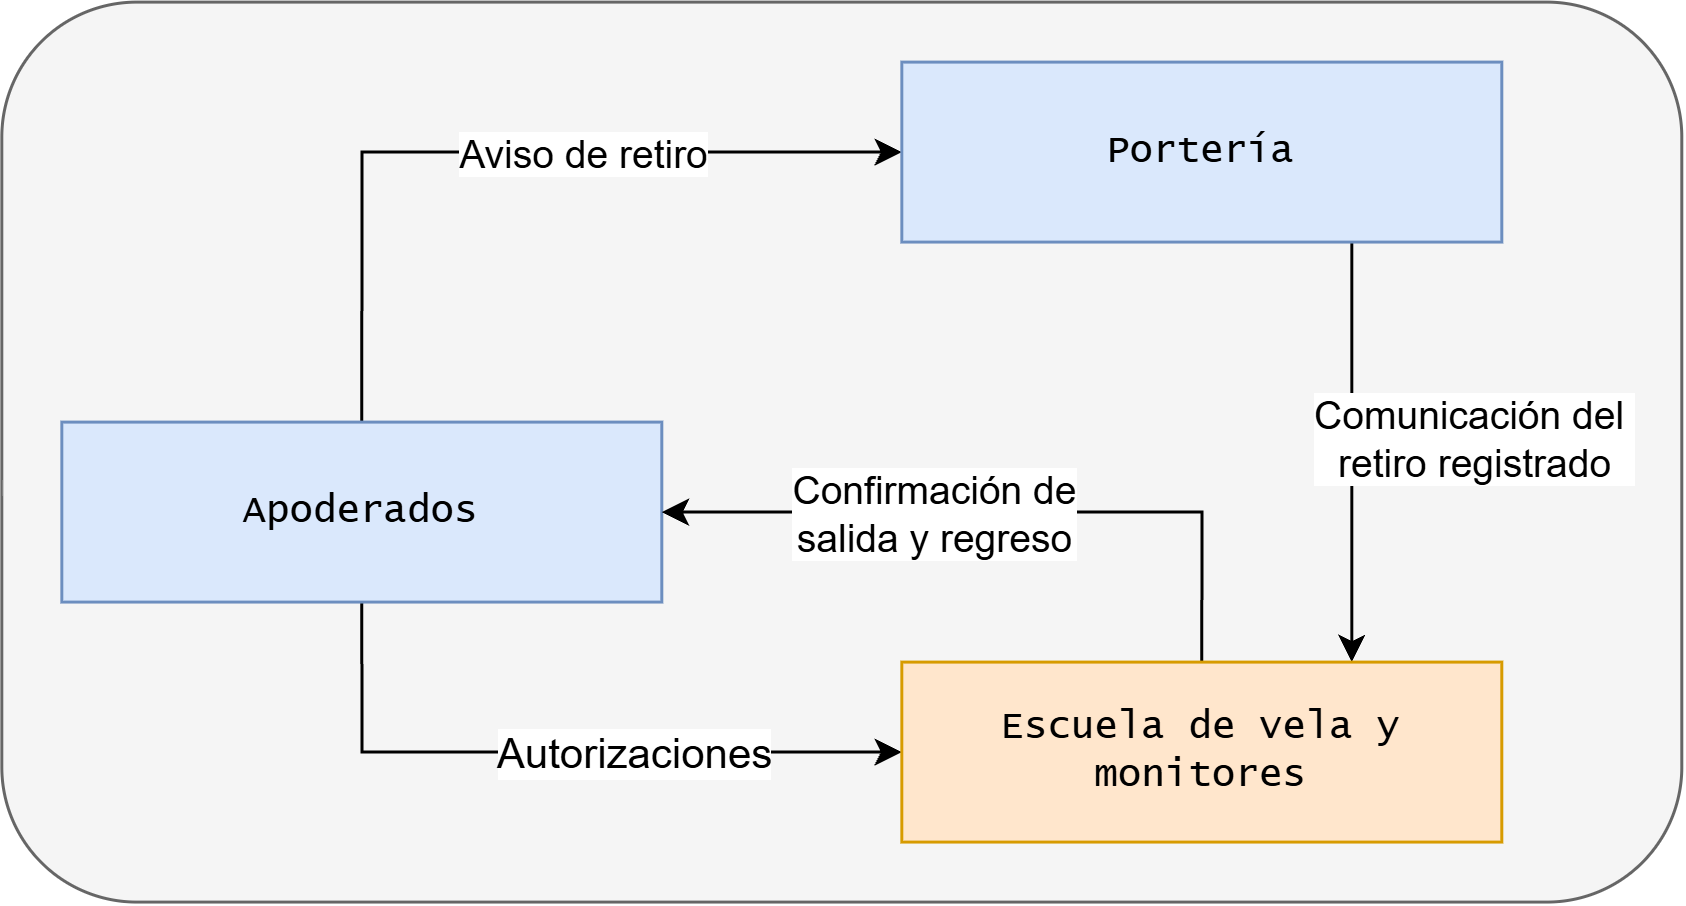
\includegraphics[width=0.75\linewidth]{figuras/ActoresEscuela.png}
    \caption{Relaciones de información de la escuela de vela}
    \label{fig:actores_escuela}
    \par\fontsize{9}{12}\selectfontskip
    \begin{minipage}{0.9\linewidth}
        \fontsize{9}{12}\selectfont
        \textit{Brecha documentada:} en el incidente de enero de 2026, el retiro quedó registrado en portería pero el aviso no llegó a la escuela. \par\fontsize{9}{12}\selectfontskip \FuenteFigura{\parencite[cap.~1, p.~4; cap.~4, secc.~4.9, p.~12]{pucv-caso07-2026}.}
    \end{minipage}
\end{figure}
El apoderado, portería y la escuela aportan antecedentes de actividades distintas, ninguno reemplaza a los demás. La relación entre ellos debe permitir distinguir autorización, presencia en el recinto, salida al agua y regreso.

\newpage
La Figura~\ref{fig:actores_operacion_maritima} distingue los antecedentes declarados por el armador de las observaciones del personal de pantalán y de la coordinación realizada por la torre.

\begin{figure}[htbp]
    \centering
    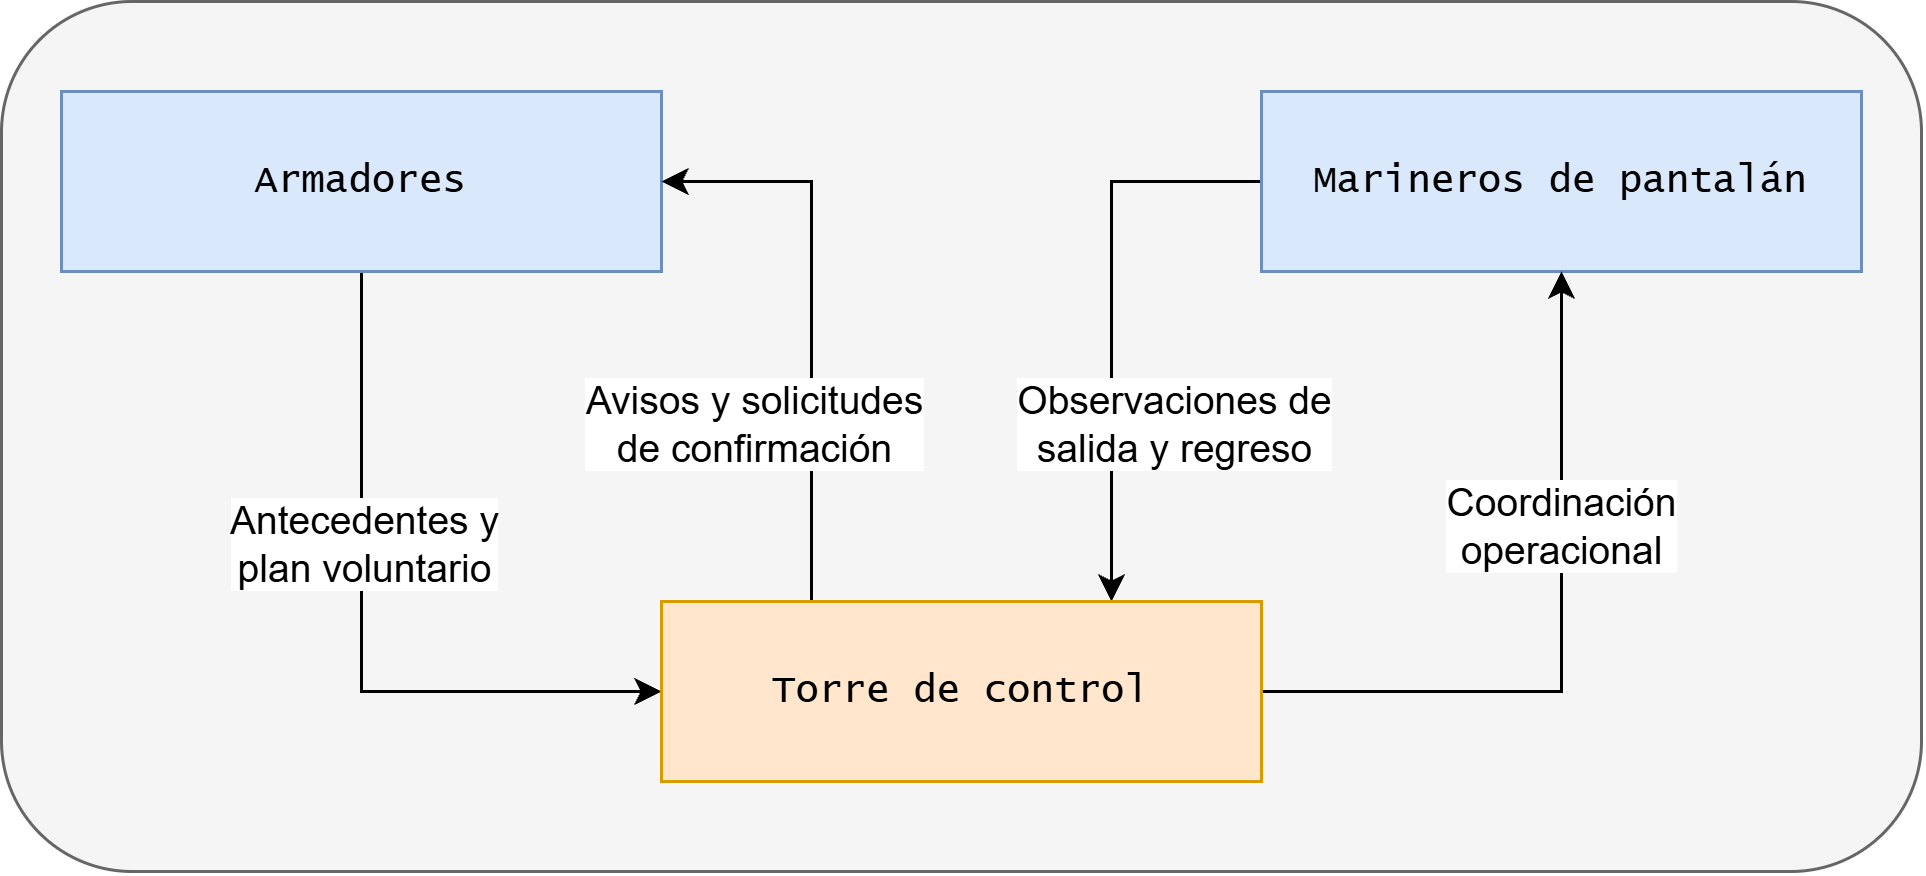
\includegraphics[width=0.85\linewidth]{figuras/ActoresOperacionMaritima.png}
    \caption{Relaciones de información de las embarcaciones}
    \label{fig:actores_operacion_maritima}
    \par\fontsize{9}{12}\selectfontskip
    \begin{minipage}{0.9\linewidth}
        \fontsize{9}{12}\selectfont
        \textit{Brecha documentada:} los regresos no se registran y los planes voluntarios se archivan sin seguimiento. \par\fontsize{9}{12}\selectfontskip \FuenteFigura{\parencite[cap.~4, seccs.~4.3-4.4, p.~10]{pucv-caso07-2026}.}
    \end{minipage}
\end{figure}

En la operación marítima, el armador entrega antecedentes de la embarcación y un plan de navegación. La torre de control coordina la operación y el personal de pantalán observa los hechos en terreno. Sus aportes tienen diferente alcance: una declaración del armador y una observación presencial deben conservar su origen, especialmente cuando existe una discrepancia. La responsabilidad de revisar esa diferencia debe quedar definida.

La Figura~\ref{fig:actores_respaldo_servicios} relaciona la evidencia operacional con las condiciones de cobro y la revisión del cliente.

\begin{figure}[htbp]
    \centering
    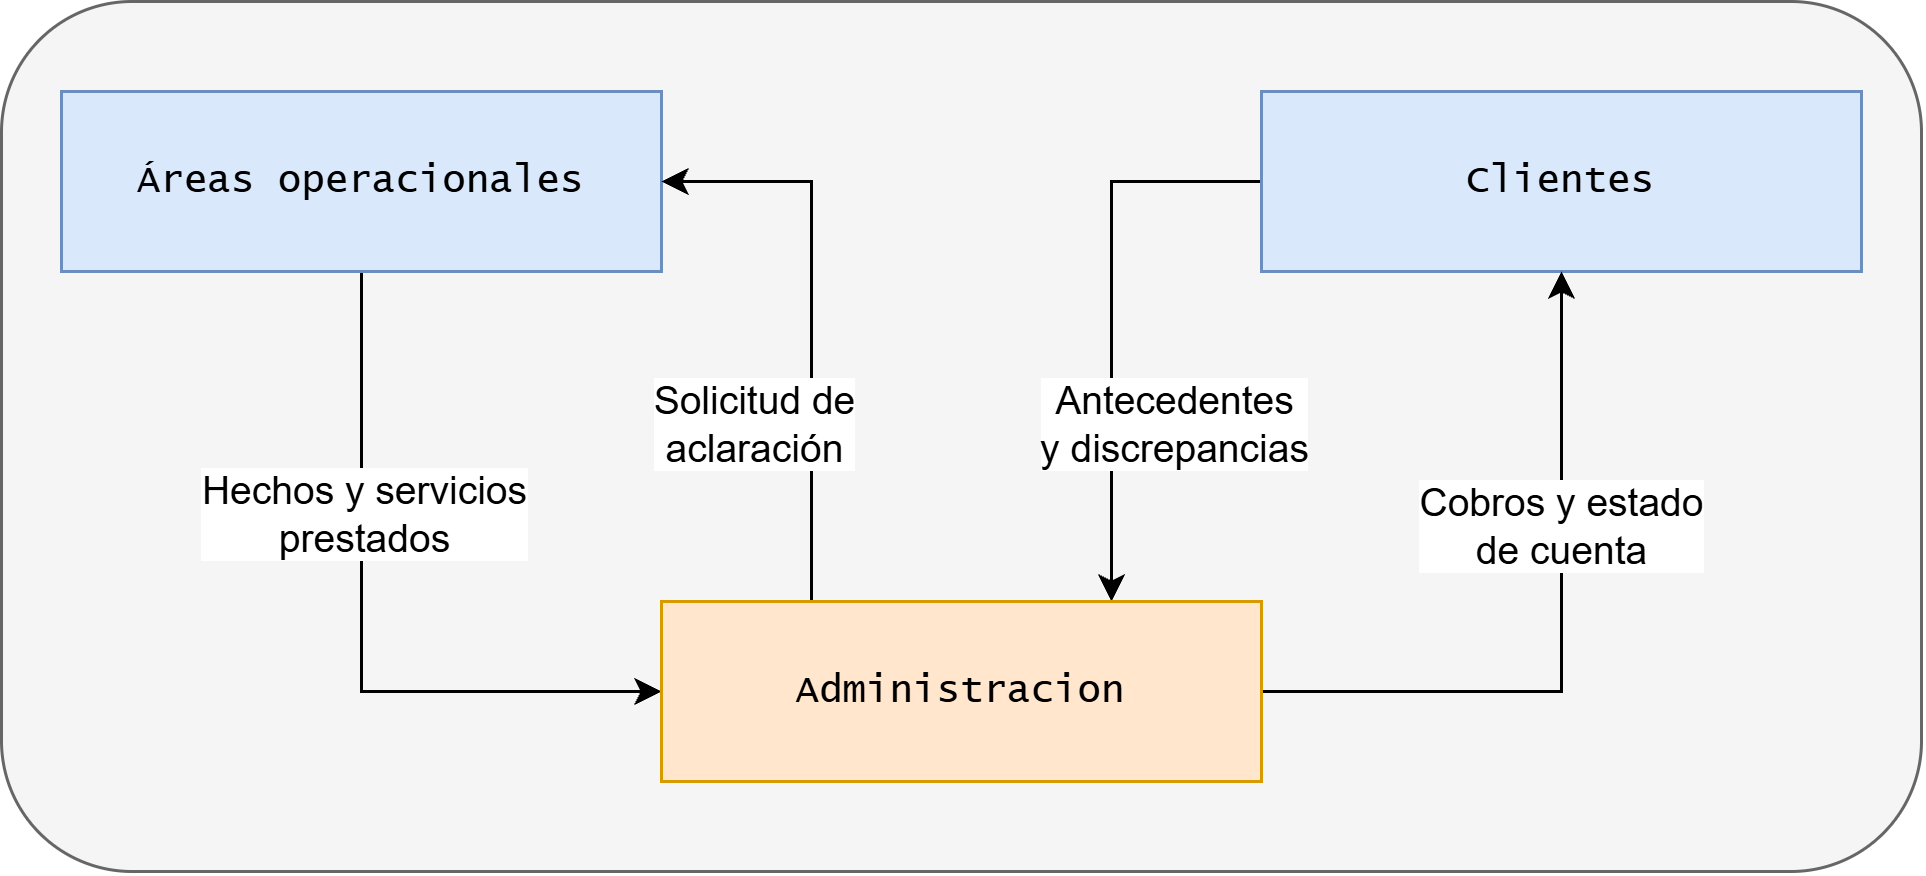
\includegraphics[width=0.85\linewidth]{figuras/ActoresRespaldoServicios.png}
    \caption{Relaciones de información del respaldo de servicios y cobros}
    \label{fig:actores_respaldo_servicios}
    \par\fontsize{9}{12}\selectfontskip
    \begin{minipage}{0.9\linewidth}
        \fontsize{9}{12}\selectfont
        \textit{Brecha documentada:} administración reúne manualmente antecedentes dispersos para facturar, con omisiones y correcciones posteriores. \par\fontsize{9}{12}\selectfontskip \FuenteFigura{\parencite[cap.~4, seccs.~4.1-4.2, pp.~9-10; secc.~4.11, pp.~12-13]{pucv-caso07-2026}.}
    \end{minipage}
\end{figure}


\newpage
La relación entre operación y administración permite respaldar servicios y estados de cuenta. Las áreas operacionales conocen qué actividad ocurrió, administración dispone de contratos y condiciones de cobro, y el cliente puede revisar los cargos y plantear diferencias. La conexión continua entre esos antecedentes permite reconstruir el servicio sin que una sola persona conozca todo el proceso.

La trazabilidad ambiental incorpora una cadena similar: los contratistas aportan antecedentes sobre los residuos, el varadero controla su recepción y el gestor autorizado acredita la entrega correspondiente. La evidencia debe relacionar esas actuaciones para su revisión por el certificador o la autoridad \parencite[cap.~4, secc.~4.7, p.~11; cap.~12, pp.~27-28]{pucv-caso07-2026}.

Estas relaciones muestran que la responsabilidad no se resuelve otorgando a todos los actores acceso a toda la información. Cada participante necesita los antecedentes pertinentes para su función, junto con un mecanismo de comunicación de cambios de estado y discrepancias. En especial, la información de salud, los datos de menores y los antecedentes de deuda requieren un tratamiento diferenciado conforme a las exigencias del caso \parencite[cap.~15, RT-11.10 y RT-16.09, pp.~34-35]{pucv-caso07-2026}.

\subsection{Intereses en tensión y necesidades de participación} %2.4.3
Las entrevistas incorporadas en las bases muestran tensiones entre objetivos legítimos de distintos participantes. Identificarlas permite evitar que una solicitud individual pueda convertirse en una regla para toda la organización. Los siguientes aspectos requieren una definición consistente con las restricciones del cliente y con las responsabilidades de cada actor \parencite[cap.~8, pp.~18-23; cap.~10, p.~26]{pucv-caso07-2026}.

\begin{itemize}
    \item \textbf{Seguridad operacional y privacidad de los armadores:}
    Operaciones necesita confirmar salidas y regresos, mientras los armadores rechazan el seguimiento de su posición sin consentimiento. Conocer un cambio de estado debe distinguirse de la vigilancia durante la navegación. La participación voluntaria en un plan de navegación tampoco puede convertirse en una obligación encubierta.
    
    \item \textbf{Control de alumnos y protección de su información:}
    La escuela y los apoderados requieren conocer la participación y el regreso, pero rechazan cámaras sobre los alumnos y dispositivos en las embarcaciones menores. El cuidado de un alumno no justifica exponer su ficha completa a todo el personal.
    
    \item \textbf{Trazabilidad y seguridad durante las maniobras:}
    Administración y las jefaturas necesitan evidencia, pero los marineros y operadores no pueden interrumpir un amarre o izaje para registrar datos. La oportunidad del registro debe definirse con quienes realizan la tarea, respetando la prohibición de exigir interacción durante la maniobra.
    
    \item \textbf{Control ambiental y capacidad de los contratistas:}
    La marina necesita asociar residuos y acreditaciones a los trabajos. El encargado advierte resistencia a instalar y utilizar una aplicación. Esta condición debe considerarse al definir la participación de los contratistas, sin eliminar las funciones de portal y declaración exigidas.
    
    \item \textbf{Cobranza, custodia y gobierno societario:}
    Administración busca medidas frente a la mora, pero restringir el acceso a una embarcación exige una decisión formal, registrada y fundada de la compañía. La condición de accionista de algunos deudores agrega una tensión de gobierno que no corresponde resolver mediante un bloqueo automático.
    
    \item \textbf{Mejora del servicio y capacidad de operación:}
    Los clientes requieren atención ágil y evidencia confiable. La gerencia debe asegurar que la marina pueda sostener el cambio sin un área TI, con responsabilidades funcionales viables y soporte técnico especializado.
\end{itemize}

La participación necesaria debe responder a estas diferencias. Gerencia y directorio deben intervenir en políticas y responsabilidades; las jefaturas, en reglas de negocio y criterios de validación; y el personal de terreno, en la viabilidad de los procedimientos. Los apoderados y representantes de clientes aportan la perspectiva de quienes reciben el servicio, mientras las autoridades, aseguradoras y certificadores permiten precisar la evidencia requerida en sus ámbitos.

El nivel de influencia no debe utilizarse como criterio único para priorizar necesidades. La baja capacidad de decisión de los alumnos no reduce la prioridad de su protección, ni la influencia de otro actor permite desplazar una restricción de seguridad o privacidad. Este análisis fundamenta la identificación de requerimientos del apartado~\ref{sec:requerimientos_supuestos} y la estrategia de participación que se desarrolla junto con la solución en el Subdocumento 3.


%---------------------------------------
\newpage
\section{Resumen de Requerimientos, Supuestos, Exclusiones y Restricciones} %2.5
\label{sec:requerimientos_supuestos}

Este apartado sintetiza las exigencias que se desprenden del diagnóstico y de las bases del proyecto. Se distingue entre requerimientos, que expresan capacidades o resultados verificables; supuestos, que permiten formular la propuesta ante información incompleta; exclusiones, que delimitan actividades no solicitadas; y restricciones, que establecen condiciones obligatorias. La distinción evita presentar una decisión del proponente como un hecho del cliente o utilizar un supuesto para reducir una obligación establecida.

El detalle está en el archivo \texttt{SYNAPTIX-Subdocumento2-Anexos.pdf}, mediante los listados de requerimientos y de supuestos, exclusiones y restricciones.

\subsection{Síntesis de requerimientos del cliente} %2.5.1

Las expectativas definidas en el caso deben traducirse en requerimientos verificables. Traducir la expectativa de conocer quién regresó requiere precisar qué hecho se registra, quién lo aporta y cómo se reconoce una situación sin confirmar. La síntesis funcional comprende los siguientes ámbitos \parencite[cap.~9, pp.~24-25; cap.~15, RT-16.30, p.~35 y RT-17.01, p.~36; cap.~18, pp.~44-45]{pucv-caso07-2026}:

\begin{itemize}
    \item \textbf{Estado de embarcaciones y gestión de amarras:} Registrar y consultar ocupación, asignaciones, reservas, salidas y regresos. Considerar las condiciones de compatibilidad del puesto y relacionar los cambios de disponibilidad con la lista de espera y los compromisos existentes.
    \item \textbf{Navegación y preparación del zarpe:} Reutilizar antecedentes de embarcaciones, armadores, patrones y documentación vigente. Conservar evidencia de su preparación y gestionar la declaración voluntaria de planes de navegación y la advertencia de vencimientos sin cierre, respetando las atribuciones de la autoridad marítima.
    \item \textbf{Avisos y contingencias:} Mantener contactos vigentes y registrar destinatarios, canales, envíos, acuses, instrucciones y escalamiento de avisos. La evidencia debe permitir distinguir un envío de un contacto confirmado y de una autorización de intervención.
    \item \textbf{Escuela de vela:} Relacionar autorizaciones, asistencia, retiros, salidas, embarcaciones, monitores y regresos. La información debe permitir establecer la participación efectiva de los alumnos y comunicar los cambios relevantes a quienes corresponda.
    \item \textbf{Varadero, invernada y boyas:} Programar maniobras considerando clima y dependencias físicas, conservar planes de izaje y sus validaciones, y registrar estado, ocupación e inspecciones de boyas y trenes de fondeo.
    \item \textbf{Servicios, consumos y control administrativo:} Vincular despachos de combustible, estadías y demás prestaciones con sus antecedentes facturables. Relacionar consumos con amarras, mantener estados de cuenta, y respaldar la gestión de mora y los expedientes de embarcaciones abandonadas.
    \item \textbf{Contratistas y gestión ambiental:} Controlar acreditaciones y vigencias, conservar evidencia de capacitación ambiental y trazar residuos desde su embarcación de origen hasta la entrega al gestor autorizado. Los registros deben sustentar los indicadores y la revisión de las no conformidades.
    \item \textbf{Atención y acceso a servicios:} Proporcionar la información pública y las funciones autenticadas exigidas para visitantes, armadores, apoderados y contratistas, incluyendo reserva y pago de amarras de visita, consulta de antecedentes y comunicaciones en los idiomas establecidos por el caso.
\end{itemize}

Estos ámbitos se relacionan entre sí. El estado de una embarcación afecta la disponibilidad de puestos, los avisos y la atención del armador, el registro de un servicio respalda su facturación y la medición de consumos sirve tanto al control económico como a la evidencia ambiental. Por ello, los requerimientos deben mantener correspondencia entre procesos y evitar definiciones contradictorias de un mismo hecho.

La Tabla~\ref{tab:umbrales_operacionales} presenta los umbrales de las transacciones críticas. Estos valores son exigencias del caso y no resultados medidos ni metas definidas libremente por Synaptix.

\begingroup
\setlength{\tabcolsep}{3pt}

\begin{longtable}{@{}L{.46\textwidth}>{\raggedleft\arraybackslash}p{.18\textwidth}L{\dimexpr.36\textwidth-12pt\relax}@{}}
    \caption{Umbrales de tiempo exigidos para las transacciones críticas}
    \label{tab:umbrales_operacionales}\\
    \hline
    \EncabezadoTabla{Operación} & \EncabezadoTabla{Tiempo máximo} & \EncabezadoTabla{Alcance de la medición} \\
    \hline
    \endfirsthead
    \hline
    \EncabezadoTabla{Operación} & \EncabezadoTabla{Tiempo máximo} & \EncabezadoTabla{Alcance de la medición} \\
    \hline
    \endhead
    Asignación y confirmación de amarra a visitante & 45 segundos & Desde la consulta \\ \addlinespace \hline
    Registro de salida o regreso en pantalán & 10 segundos & Máximo dos interacciones \\ \addlinespace \hline
    Preparación de nómina y antecedentes de zarpe & 90 segundos & Conformación del legajo \\ \addlinespace \hline
    Registro de salida de una clase de vela & 60 segundos & Hasta 18 embarcaciones \\ \addlinespace \hline
    Notificación de emergencia a 296 armadores & 10 minutos & Hasta el último envío \\ \addlinespace \hline
    Alerta por plan vencido sin cierre & 15 minutos & Desde su vencimiento \\ \addlinespace \hline
\end{longtable}

\FuenteTabla{\parencite[cap.~15, RT-09.01, p.~34]{pucv-caso07-2026}.}
\endgroup

La interpretación de los umbrales es parte de los requerimientos. El tiempo de preparación del legajo no corresponde al otorgamiento del zarpe, el plazo hasta el último envío no garantiza que todos los armadores hayan acusado recibo y el registro de una salida no puede exigirse durante una maniobra. Las pruebas y los criterios de aceptación deberán conservar estos límites para evitar demostrar una operación distinta a la solicitada.

Además de los tiempos de ejecución de las transacciones, el caso exige una actualización diferenciada de la información operacional: la ocupación de una amarra debe actualizarse en un máximo de 60 segundos desde el evento, el consumo acumulado por amarra al menos cada hora, el estado de cuenta del armador y la situación de la escuela de vela en tiempo real, y los indicadores ambientales mediante consolidación diaria. Estas condiciones complementan los límites de la Tabla~\ref{tab:umbrales_operacionales} y deben conservarse en los criterios de aceptación \parencite[cap.~15, RT-05.29, p.~34]{pucv-caso07-2026}.

La continuidad requiere sostener al menos 24 horas de operación del recinto sin enlace exterior en los procesos indicados por RT-03.10, 12 horas sin cobertura para los dispositivos de terreno de pantalán, varadero y escuela, y 8 horas para la inspección de boyas. Tras 24 horas de desconexión, la sincronización no debe superar 30 minutos ni requerir intervención manual, y debe preservar los registros críticos establecidos. Estos plazos corresponden a contextos diferentes y no deben unificarse bajo una sola autonomía genérica \parencite[cap.~15, RT-03.10 y RT-03.13, p.~33]{pucv-caso07-2026}.

La gestión de información debe contemplar las retenciones diferenciadas de RT-05.10, el resguardo de datos personales y de salud, el registro de consultas a información sensible y las firmas exigidas para las actuaciones indicadas por las bases. La conservación histórica no se limita a almacenar documentos sino que también debe  permitir recuperarlos y relacionarlos con el hecho, persona o embarcación correspondiente \parencite[cap.~15, RT-05.10, RT-11.10, RT-16.09 y RT-16.14, pp.~33-35]{pucv-caso07-2026}.

La migración debe incluir la totalidad de socios y armadores, los contratos de amarra vigentes y su documentación, seis años de pagos y saldos, los antecedentes completos de las 14 embarcaciones abandonadas, la totalidad del registro de embarcaciones e invernadas y la matrícula de la escuela de los últimos tres años. La antigüedad del sistema de origen no autoriza a sustituir este alcance por una migración indiscriminada de doce años ni a omitir antecedentes por su dificultad de extracción \parencite[cap.~15, RT-05.15, p.~34]{pucv-caso07-2026}.

En atención y operación se exigen el portal y los cinco perfiles móviles del caso, así como interfaces adecuadas a las condiciones de terreno. Los cinco perfiles móviles exigidos responden a funciones y condiciones de uso diferentes \parencite[cap.~10, p.~26; cap.~15, RT-13.08, p.~35 y RT-17.01, p.~36]{pucv-caso07-2026}.
%

\begin{itemize}
    \item \textbf{Marinero de pantalán:} Registro de salidas y regresos de embarcaciones, con operación mediante guantes, un máximo de dos interacciones por registro y funcionamiento sin conexión. Su uso debe respetar la prohibición de interactuar durante la maniobra.

    \item \textbf{Monitor de la escuela de vela:} Preparación y cierre de las salidas al agua, relacionando alumnos, embarcaciones y monitores para establecer la participación y confirmar el regreso.

    \item \textbf{Varadero:} Consulta y registro de antecedentes de la maniobra y del plan de izaje. El plan debe estar disponible antes de la ejecución, sin exigir interacción con dispositivos mientras exista una carga suspendida.

    \item \textbf{Inspección del campo de boyas:} Registro del estado y ocupación de las boyas y de las inspecciones de sus trenes de fondeo, con operación totalmente desconectada durante el trabajo en terreno.

    \item \textbf{Armador:} Declaración y cierre voluntario del plan de navegación, con un modo de comunicación de baja capacidad para su uso durante la navegación.
\end{itemize}

La notificación de emergencia debe utilizar al menos tres canales simultáneos: SMS, mensajería instantánea y correo, exigiendo un acuse de recibo registrado por destinatario, y se realiza una llamada a quienes no acusen. La atención del centro de servicio comprende de 06:00 a 24:00 en temporada alta y de 08:00 a 20:00 el resto del año, el canal de notificación de emergencia y la recepción de alertas de planes vencidos mantienen operación continua. Estos compromisos deben interpretarse conjuntamente con las exigencias de idioma y con la ausencia de personal TI del cliente \parencite[cap.~2, secc.~2.4, pp.~7-8; cap.~15, RT-13.12 y RT-16.21, p.~35; RT-21.06, p.~36]{pucv-caso07-2026}.

Para las embarcaciones en navegación, se exige un canal de comunicación de baja capacidad, tolerante a latencias de horas y a la recepción de mensajes fuera de orden. El perfil móvil del armador debe contemplar este modo para la declaración y el cierre de su plan de navegación. Esta capacidad debe respetar la participación voluntaria y las condiciones de consentimiento del caso \parencite[cap.~15, RT-16.21 y RT-17.01, pp.~35-36]{pucv-caso07-2026}.

La prioridad de seguridad expresada por el cliente orienta el análisis, pero no elimina los demás requerimientos ni determina por sí sola la distribución entre etapas. La evidencia ambiental necesita tiempo de acumulación antes de la temporada 2029, y el control de regresos depende de una definición confiable del estado de las embarcaciones. La secuencia de implementación deberá considerar esas dependencias en el Subdocumento 3 y en el plan de trabajo, sin convertir el orden de preferencia en una exclusión de alcance \parencite[cap.~13, pp.~28-29]{pucv-caso07-2026}.

\subsection{Supuestos y tratamiento de la incertidumbre} %2.5.2
Un supuesto permite formular una propuesta cuando un antecedente no está completamente determinado. Debe expresar qué se considera, por qué resulta razonable y qué consecuencia tendría que no se cumpla. No corresponde presentar como supuesto una restricción ya establecida, como la ausencia de personal TI o la continuidad del sistema contable, ni presumir la existencia de interfaces, datos depurados o infraestructura que las bases no acreditan.

Para la formulación del proyecto, se declaran los siguientes supuestos de trabajo. Su validación no equivale a trasladar al cliente las obligaciones técnicas del adjudicatario, permite precisar las condiciones de colaboración y ajustar las decisiones que dependan de ellas.

\begin{enumerate}
    \item \textbf{Disponibilidad de representantes funcionales (SUP-01):} Se supone que la gerencia coordinará la participación de representantes de operaciones, administración, escuela y varadero para revisar reglas de negocio y validar resultados en sesiones programadas. El fundamento es que esas áreas poseen el conocimiento operacional y la autoridad funcional necesarios. No se presume dedicación exclusiva ni capacidad técnica especializada, su disponibilidad debe precisarse al organizar el trabajo.

    \item \textbf{Acceso autorizado a fuentes (SUP-02):} Se supone que el cliente facilitará el acceso controlado a los registros y documentación que mantiene bajo su custodia, incluyendo el sistema administrativo y los expedientes físicos. Este supuesto no implica que los datos estén completos, depurados o sean exportables directamente. Su calidad y estructura deben comprobarse mediante el análisis de las fuentes.

    \item \textbf{Volumetría como referencia de estimación (SUP-03):} Para formular las estimaciones iniciales, se considera que los volúmenes y escenarios del caso son representativos de la operación que debe soportar la solución. Su conversión a usuarios concurrentes, transacciones, mensajes y almacenamiento requiere hipótesis explícitas por proceso. Estas hipótesis deben contrastarse con antecedentes verificados, manteniendo separados la actividad habitual, los períodos de máxima demanda y los escenarios de crecimiento.

    \item \textbf{Compras y obras a cargo del cliente (SUP-04):} Para planificar la instalación e integración, se supone que las adquisiciones y obras asignadas al cliente podrán estar disponibles en los hitos que se acuerden a partir de especificaciones oportunas del proponente. No se presume que estén ejecutadas al inicio del proyecto. Las fechas necesarias y condiciones de recepción deben incorporarse como dependencias del cronograma; un incumplimiento exige revisar sus efectos y alternativas, sin asumir una extensión automática de los plazos.

    \item \textbf{Aprobación de decisiones de negocio (SUP-05):} Se supone que la compañía podrá designar a quienes aprueben criterios comerciales y operacionales, como priorización de la lista de espera o las autorizaciones excepcionales. Se debe formular criterios y analizar sus consecuencias, pero no atribuirse decisiones societarias o actos que corresponden al cliente.
\end{enumerate}

Si alguno de estos supuestos no se cumple, debe identificarse qué actividad resulta afectada y qué alternativa permite mantener los compromisos aplicables. Por ejemplo: la falta de documentación del sistema de origen incrementa el trabajo de análisis, pero no elimina la obligación de migración. Del mismo modo, la participación limitada de una jefatura requiere organizar la validación y sus respaldos, sin asumir que el silencio equivale a aprobación.

El registro de supuestos de A2.3 incluye también las 22 decisiones que el proponente debe formular para el caso, identificadas como DEC-01 a DEC-22. Cada una explicita el criterio asumido para la propuesta, su fundamento, el impacto si resulta equivocado y la instancia prevista de validación \parencite[cap.~16, secc.~16.1, pp.~36-38; cap.~17, secc.~17.1, p.~40]{pucv-caso07-2026}. A continuación se resumen cuatro criterios relevantes para la seguridad operacional y la continuidad de la gestión.

\begin{itemize}
    \item \textbf{Estado y regreso de las embarcaciones (DEC-01 y DEC-05):} Se propone mantener separado el estado operacional registrado, la declaración del armador y las discrepancias entre ambos. La confirmación del regreso al recinto requiere una observación identificada de la embarcación amarrada en condición segura; el cierre del plan voluntario no acredita por sí solo ese regreso.

    \item \textbf{Conciliación de retiros de alumnos (DEC-07):} Se propone vincular el retiro registrado en portería con el control de participación de la escuela, distinguiendo la solicitud de retiro de la entrega confirmada. Un retiro confirmado debe impedir una nueva confirmación de salida del alumno. Si no puede comprobarse el estado vigente por una falla de comunicación, debe aplicarse el procedimiento de contingencia y conservar evidencia para su conciliación posterior.

    \item \textbf{Alcance del plan voluntario de navegación (DEC-04):} Se propone conservar la declaración y el cierre del plan como antecedentes independientes de la confirmación operacional de regreso. El vencimiento sin cierre genera la alerta dentro del plazo exigido y requiere atención identificada, sin atribuir a la marina funciones de búsqueda y salvamento ni convertir el plan voluntario en obligatorio.

    \item \textbf{Administración funcional de la solución
    (DEC-22):} Se propone una administración funcional compartida: el cliente conserva la aprobación de las políticas de negocio y el adjudicatario proporciona asistencia funcional y las tareas especializadas comprometidas. Su desarrollo debe precisar actividades, responsables, dedicación y suplencias, sin suponer que la marina dispone de personal TI propio.
\end{itemize}

Esta síntesis no reemplaza el registro completo de A2.3. En SD2 se explicitan los criterios asumidos y sus condiciones de validación. SD3 desarrolla los flujos, responsabilidades funcionales y excepciones. SD4 y SD5 desarrollan las implicancias de arquitectura y datos. Los parámetros o antecedentes pendientes deben identificarse expresamente, sin presentar una validación futura como realizada ni sustituir el criterio propuesto por una remisión genérica a otro subdocumento.

En particular, no se presume que un sistema externo disponga de una interfaz automatizada sólo porque las bases exijan intercambio de información. Debe verificarse la disponibilidad efectiva de los formatos y canales correspondientes. Esa verificación condiciona el mecanismo de integración, pero no modifica las atribuciones de la autoridad ni permite omitir el intercambio exigido \parencite[cap.~15, RT-05.23, p.~34]{pucv-caso07-2026}.

\subsection{Exclusiones y obligaciones} %2.5.3

Las exclusiones delimitan actividades que el cliente no solicita al adjudicatario. Sin embargo, una actividad excluida puede generar información o dependencias necesarias para el proyecto. Por ello, debe indicarse tanto lo que queda fuera como la obligación de integración, especificación o respaldo que permanece \parencite[cap.~11, pp.~26-27]{pucv-caso07-2026}.

\begin{itemize}
    \item \textbf{Sistema contable y documentos tributarios:} Se excluye su reemplazo y la sustitución de la emisión tributaria. Se mantiene la obligación de proporcionar los hechos facturables y de considerar la relación con el sistema existente.
    
    \item \textbf{Sistema y acto de la autoridad marítima:} Se excluye desarrollar o sustituir el sistema de zarpe de la autoridad. Permanece la preparación, validación y trazabilidad de antecedentes dentro de los formatos y canales aplicables.
    
    \item \textbf{Remuneraciones y administración de personal:} No forman parte de la gestión solicitada. Esta exclusión no elimina la identificación de usuarios, funciones y habilitaciones necesaria para utilizar los servicios.
    
    \item \textbf{Cobranza judicial y actuaciones sobre embarcaciones abandonadas:} Se excluye operar esos procedimientos. Permanece la construcción y conservación del expediente trazable que permita al cliente adoptar las actuaciones correspondientes.
    
    \item \textbf{Administración del restaurante y su punto de venta:} Se excluye su gestión interna. Se mantiene el registro de su relación contractual y de los consumos de servicios que correspondan a la marina.
    
    \item \textbf{Ejecución de obras físicas y adquisición del hardware indicado en el caso:} Las obras y compras asignadas al cliente no son ejecutadas por el proponente. Permanecen la especificación de cantidades, características y condiciones de instalación, la consideración de sus costos en los documentos económicos correspondientes y la gestión de sus dependencias para la integración.
    
    \item \textbf{Certificación ambiental de la marina:} No se ofrece otorgar la certificación. Se mantienen las capacidades de registro y evidencia necesarias para atender las no conformidades y sostener los indicadores exigidos.
    
    \item \textbf{Instrumentación de embarcaciones de armadores:} Se excluye proveer equipamiento de a bordo o instrumentar sus embarcaciones. Las funciones voluntarias de declaración y comunicación deberán respetar esta delimitación y las condiciones de consentimiento.
    
    \item \textbf{Mantención física de boyas y trenes de fondeo:} Se excluye realizar esa mantención. Permanece el registro del estado, ocupación y cumplimiento del programa de inspección.
\end{itemize}

Estas delimitaciones no constituyen una exención general sobre los procesos relacionados. Por ejemplo: que el cliente compre un medidor no elimina la obligación de especificar su compatibilidad e integración, que el certificador sea un tercero no permite omitir la evidencia ambiental y que el sistema contable se mantenga no resuelve por sí solo la calidad de los antecedentes que recibe.

El plan y la gestión de riesgos deben considerar las dependencias generadas por obras, adquisiciones, sistemas externos y actuaciones de terceros. Tampoco corresponde ampliar por analogía las exclusiones del hardware de terreno a toda provisión tecnológica de la propuesta, cada responsabilidad debe conservar el alcance que le asignan las bases aplicables.

\subsection{Restricciones obligatorias y consecuencias} %2.5.4

Las restricciones limitan las alternativas admisibles y deben mantenerse presentes en el alcance, el diseño y la operación. No son preferencias que puedan descartarse por conveniencia técnica, corresponden a condiciones no negociables del cliente y a parámetros específicos del caso. Su síntesis se organiza según el efecto que producen sobre el proyecto \parencite[cap.~10, p.~26; cap.~15, pp.~33-36]{pucv-caso07-2026}.

\begin{itemize}
    \item \textbf{Seguridad de las maniobras:} Ninguna función puede retrasar o interferir un amarre o izaje, ni exigir interacción con un dispositivo durante su ejecución. Los procedimientos de captura deben respetar el momento seguro de trabajo.
    \item \textbf{Privacidad y participación voluntaria:} No se instalarán dispositivos de seguimiento en embarcaciones de armadores sin consentimiento expreso. Las funciones que dependan de datos aportados por el armador deben respetar la voluntariedad y la revocación del consentimiento.
    \item \textbf{Protección de alumnos:} No se utilizarán cámaras dirigidas a los alumnos ni dispositivos a bordo de las embarcaciones menores. Los datos de salud y los datos personales de menores deben quedar disponibles sólo para quienes los necesitan en su actividad.
    \item \textbf{Medios y atribuciones existentes:} La radio marítima se mantiene, el zarpe conserva su autoridad y formato y el sistema contable sigue siendo el único emisor de documentos tributarios. La propuesta debe convivir con estos elementos. 
    \item \textbf{Operación sin personal TI del cliente:} Las funciones que requieran especialistas deben ofrecerse como servicio durante los 36 meses de operación. La administración funcional no puede utilizarse para trasladar tareas técnicas a personal sin esa capacidad.
    \item \textbf{Continuidad y condiciones de terreno:} Los procesos críticos deben continuar sin enlace exterior conforme a sus autonomías exigidas. El equipamiento de pantalanes debe acreditar aptitud para estructuras flotantes y ambiente marino y el instalado en el surtidor debe acreditar idoneidad para la clasificación del recinto.
    \item \textbf{Idioma y accesibilidad operacional:} Deben respetarse las exigencias del idioma y las condiciones de uso de los perfiles reales, incluyendo guantes, humedad, exposición solar y trabajo fuera de cobertura.
    \item \textbf{Cobranza y acceso a bienes en custodia:} No puede impedirse el acceso de un armador a su embarcación mediante una medida de cobranza sin una decisión formal, registrada y fundada de la compañía. La automatización no sustituye esa autorización.
\end{itemize} 

Las ventanas de intervención constituyen otra restricción determinante. Se prohíbe intervenir sistemas entre el 15 de diciembre y el 15 de marzo, durante los eventos del calendario náutico, y en lo que afecte al varadero, durante las campañas de abril-mayo y septiembre-noviembre. Los avisos de marejadas obligan a suspender las actividades programadas conforme a las bases, el plan debe absorber esas cancelaciones sin desplazar los hitos contractuales. Por ello, instalación, pruebas, capacitación y cambios deben analizarse conjuntamente con el calendario operacional, no sólo con la disponibilidad del equipo de proyecto \parencite[cap.~10, p.~26; cap.~15, RT-10.05, p.~34 y RT-22.04, p.~36]{pucv-caso07-2026}.

Las exigencias regulatorias y los compromisos con terceros deben traducirse en controles y evidencia aplicables a cada proceso. El marco identificado incluye concesión y operación marítima, protección de datos, actividades con menores, residuos, combustibles, consumos, contratos y custodia. Mencionar una norma no acredita su cumplimiento, la correspondencia entre obligación, control y evidencia debe desarrollarse en el tratamiento normativo de la propuesta y mantenerse coherente con los registros solicitados \parencite[cap.~12, pp.~27-28]{pucv-caso07-2026}.

La revisión conjunta de requerimientos, supuestos, exclusiones y restricciones permite establecer una propuesta verificable. Los requerimientos establecen lo que debe lograrse, los supuestos hacen explícitas las condiciones no confirmadas, las exclusiones distinguen responsabilidades y las restricciones fijan los límites que deben respetarse. Su desarrollo posterior debe conservar esta separación y una trazabilidad común, para que ninguna obligación desaparezca al pasar del diagnóstico al diseño.